\chapter{Introduksjon}
\paragraph{}I kapittel 1 ønsker gruppen å ta for seg en introduksjon av prosjektet. Dette er innledningen til selve oppgaven, og her beskrives hvem prosjektgruppen er, hvem oppdragsgiveren er, hva oppdraget er, hvilke forutsetninger og rammer prosjektet har og til slutt om strukturen på rapporten. Dette er et viktig kapittel for å få med seg informasjon om bedriften og prosjektgruppen og hvorfor prosjektet ble startet.
\section{Prosjektgruppen}
\paragraph{} Prosjektgruppen består av 4 medlemmer med ulik kompetanse og interesser. Den utgjør; Thomas Ellingsen, Erhan Sanlioglu, Mostafa Aziz og Victor Garberg Minge. Gruppen fant sammen etter å ha blitt kjent med hverandre under høstsemesteret og valgte å starte dette prosjektet sammen etter å ha snakket og diskutert sammen og kommet til enighet om at dette kan være en gruppe som kan utføre et godt prosjekt.


\begin{figure}[h]
\centering

\includegraphics[width=1.5in]{Bilder/victor2.jpg}
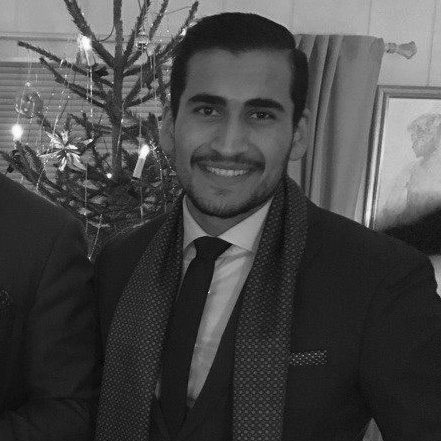
\includegraphics[width=1.5in]{Bilder/erhan2.jpg}
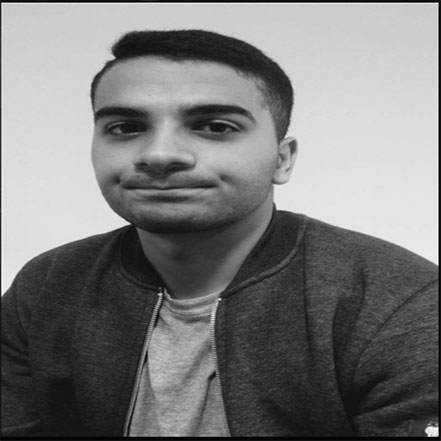
\includegraphics[width=1.5in]{Bilder/mosti2.jpg}

\includegraphics[width=1.5in]{Bilder/thomas2.jpg}
\end{figure}


\paragraph{} \textbf{Mostafa Aziz} er født den 01. november 1997, han valgte å studere informasjonssystemer på høgskolen i Østfold etter videregående skole. Mostafa har en rekke interesser deriblant datamaskiner og hvordan datamaskiner fungerer. Det å arbeide med servere var noe som interesserte Mostafa, ettersom det kunne være noe han kunne legge til som et område han kjenner til og ønsker å lære seg hvordan servere fungerer og hva som kan være relevant for fremtiden.




\paragraph{}\textbf{Thomas Ellingsen} født den 22.Juni 1995. Thomas har vært ett år i forsvaret og tatt utdanning som brannkostabel. I dag jobber han i Norskbrannvern hvor mesteparten av jobben går ut på kontroll og service av alarmanlegg. Thomas ønsker og kunne kombinere interessen for brann og redning med informasjonsteknologi. Derfor passet studiet informasjonssystemer på høgskolen i Østfold han perfekt. 

\paragraph{} \textbf{Victor Johannes Garberg Minge} er født den 04 August 1997. Victor studerer informasjonssystemer på Høgskolen i Østfold. Som ung har Victor alltid hatt stor interesse for det teknologiske, blandet med kreativitet falt han for linjen han nå går på Høgskolen. Victor har også en interesse for å løse problemer, noe som gjør IT et spennende område å arbeide og finne kreative løsninger. Som plan har Victor tenkt til å gjøre ferdig sin Bachelor på Høgskolen for å så se ann om videreutdanning eller arbeidslivet. Ellers har Victor en kjæreste og andre interesser deriblant idretten boksing og dataspill.

\paragraph{} \textbf{Erhan Mikael Sanlioglu} er født den 08 Desember 1994. Erhan studerer informasjonssystemer på høgskolen i Østfold. Med avlagt fagprøve og endt førstegangstjeneste kunne Erhan sette i gang med sine IT-studier på høgskolen. Erhan har hatt stor interesse for data i en tidlig alder og bestemte seg ganske tidlig for å ta en utdanning i dette feltet. Som fagarbeider har Erhan både arbeidserfaring fra det offentlige sektor og kunnskapen som trengs i dette fagfeltet. En kombinasjon som fagarbeider og en mastergrad i IT vil sikre fremtiden hans.

\section{Oppdragsgiver}

\begin{figure}[H]
\centering

\includegraphics[width=3.5in]{Bilder/katoplast_logo.png}
\caption{Katoplast logo}
\end{figure}


\paragraph{} Oppdragsgiver for prosjektet er daglig leder ved Katoplast AS, Trond Vidar Kjellin som har tillat en gruppe med studenter fra Høgskolen i Østfold å utføre et prosjekt i bedriften Katoplast AS.

\paragraph{} Bedriften ble grunnlagt i 1972 av Gunnar og Ivar kjellin. Bedriften driver produksjon, utforming, konstruksjon og materialvalg av plastprodukter. Plastproduksjonen skjer gjennom 3D-printing og gjennom støping av former. Katoplast har om lag 15-20 ansatte og selve produksjonen blir driftet av 14 forskjellige maskiner. \footnote{http://www.katoplast.no/produkter/}.

\paragraph{}Virksomheten har med årene flyttet flere ganger. I 1983 ble beslutningen tatt om å bygge egne lokaler i Tistedal, og disse var innflytningsklare på høsten 1984. Etter dette har det vært behov for flere utbygginger.\footnote{http://www.katoplast.no/om-katoplast/}.

\section{Oppdraget}
\paragraph{} Som oppdrag har prosjektgruppen blitt utdelt en rekke problemstillinger som gruppen skulle ha som utgangspunkt. Disse problemstillingene inkluderte alt fra å løse små, administrative oppgaver, til å finne store løsninger knyttet til ERP-system. Disse oppgavene inkluderte blant annet oppdatering av serverne, mye manuelt arbeid når det gjelder å legge inn data om kjøp og salg som har blitt gjort og annen informasjon om produkter og kunder.  I midlertid, valgte gruppen å gå for å løse serverproblemet som preger bedriften i stor grad. Oppdraget vil ta for seg flere, forskjellige sider ved ulike serverløsninger som kan være aktuelle for bedriften Katoplast AS

\paragraph{} I løpet av året 2016 har Katoplast opplevd problemer med sine servere, og hvordan deres IT-systemer generelt fungerer. Bedriften presenterte en rekke problemstillinger for gruppen som var IT-relaterte, og som gjorde at arbeidet deres i bedriften ikke ble gjort effektivt nok. Mye av problemene inkluderte høye kostnader, trege servere og manuelt arbeid som krever mye tid. Bedriften benytter seg av to ERP-system som tar for seg en rekke oppgaver innen bedriften. Access-løsningen tar seg av oppgaver knyttet til produksjonsdataen, mens en Mamut-løsning tar seg av det økonomiske regnskapet som gjennomføres. I midlertid, krever disse ERP-systemene at mye av arbeidet gjøres manuelt og dette viser seg å være et problem. Dette krever mye tid og arbeidskraft og dette fører til at mye av hovedfokuset rettes mot IT-oppgavene fremfor produseringen av varer til kunder.

\paragraph{}Gruppen diskuterte de ulike problemstillingene som ble presentert av bedriften, og som konklusjon ble resultatet å forsøke å rette, eller hjelpe Katoplast med å finne en løsning for deres serverproblem. Problemstillingene hadde et stort omfang og det var dermed rimelig å velge å fokusere på kun et av problemene fremfor alle.

\paragraph{}Situasjonen i bedriften når det gjelder servere, er at de nåværende serverne begynner å bli gamle og trege, og ikke minst skaper de problemer og utsettelser for bedriften. Prosjektets hovedfokus vil dermed legges på dette med servere og det å analysere og finne en løsning som kan være aktuell for bedriften. Katoplast ønsker en løsning som legger vekt på brukervennlighet, funksjonalitet, riktig mengde med datalagring og ikke minst en rimelig pris som kan lette på det økonomiske trykket som bedriften opplever. Gruppen må også legge vekt på fremtiden og hva som kan være enklest å håndtere for bedriften.

\begin{figure}[H]
\centering
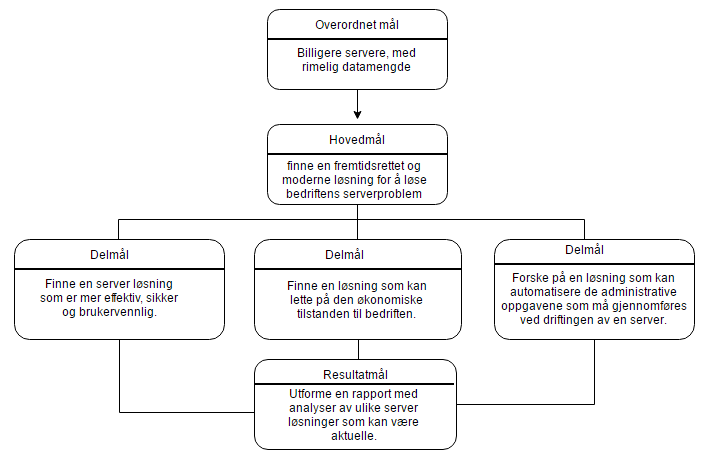
\includegraphics[width=6.5in]{Bilder/maal.PNG}
\caption{Prosjektets mål og resultatkrav}
\end{figure}

\section{Forutsetninger og rammer}

\paragraph{}Katoplast AS var åpne for at prosjektet og gruppen kunne ta fatt på oppgaven fra flere ulike vinkler, uten for mange avgrensninger og rammer som kunne eventuelt hindre sluttrapporten å oppnå beste kvalitet. Prosjekteierne ønsket ikke å begrense gruppen for mye og fokuserte hovedsakelig kun på noen små avgrensninger, som prosjektet måtte forholde seg til. Dette er svært positivt for gruppen ettersom det vil bli lettere å utforme analyser av ulike serverløsninger som kan være aktuelle for bedriften å velge. Flere muligheter vil bli dekket, og Katoplast vil kunne ha et større utvalg av løsninger når de til slutt skal velge den veien de ønsker å gå for. Katoplast var mest foukserte på sikkerhet, og var usikre når det gjaldt sky-løsninger. 

\section{Rapportstruktur}
\paragraph{} Prosjektet er delt opp i flere kapitler som tar for seg ulike områder for å skape en helhetlig rapport som er detaljert, men samtidig  enkel å forstå. Kapittel 1 av rapporten vår tar for seg introduksjonen av prosjektet. Her presenterer gruppen seg selv, oppdragsgiveren, hva oppdraget er og hva vi ønsker å oppnå og hvilke forutsetninger som er satt for prosjektet.

\paragraph{} Det neste kapittelet, kapittel 2, tar for seg teori og ulik fagstoff for prosjektet. Her beskrives vanskelig terminologi, og ulike konsepter som er viktig å forstå og vite hva er før en går videre med å lese prosjektet. Kapittel 2 er viktig for å skape et forståelig bilde av hele rapporten og de ulike analysene som er blitt gjort. Det vil finnes mange vanskelige begreper og uttrykk og teori kapittelet vil være til god hjelp for å forstå disse. I dette kapittelet beskrives de ulike delene ved servere og nettskyer, og de ulike tjenestene forklares.

\paragraph{} Det tredje kapittelet tar for seg metode. Altså hvilke metoder som ble benyttet for å finne frem til informasjon og hente ut informasjon. Den tar for seg de ulike metodene som gruppen benyttet, fra intervju til nettsøk til spørreundersøkelser. Den inkluderer også en situasjonsanalyse av bedriften for å få et bedre bilde av hvilken situasjon bedriften befinner seg i. Situasjonsanalysen er viktig for metode, ettersom den er viktig for innhentingen av informasjon for de senere analysene.

\paragraph{} Det fjerde kapittelet tar for seg de mange resultatene som gruppen har kommet til etter å ha gjennomført metodene, og med en situasjonsanalyse i bakhode. Her tar prosjektet for seg en arbeidskravsanalyse for å forstå hva som bør legges vekt på i analysene av de ulike løsningene, samt de mange resultatene som følge av forskningen som ble gjort på de ulike løsningene som gruppen har valgt å fokusere på. Her finner man resultatene av spørreundersøkelsen og et diagram som viser prisen på de ulike løsningene. 

\paragraph{} Kapittel 5 er diskusjonsdelen og diskuterer de ulike løsningene opp mot arbeidskravsanalysen og situasjonsanalysen som har blitt dannet. Diskusjons delen tar for seg de ulike løsningene for interne servere, sky tjenester og hybride løsninger som er viktige for Katoplast å vite. Dette er den viktigste delen av prosjektet ettersom den tar for seg hvordan de ulike løsningene kan påvirke Katoplast sin situasjon, og hvilken pris hver og en av de har.

\paragraph{} Avslutningsvis, så kommer konklusjonen som er det sjette og siste kapittelet. Konklusjonen tar for seg avslutningen på rapporten og vil komme med en anbefaling på hvilken løsning prosjektgruppen mener er den beste for bedriften Katoplast. Konklusjonen vil oppsummere hele prosjektet og prosjektgruppen vil ta et valg ut i fra den forskningen og de resultatene som gruppen har samlet sammen. 
\footnote{https://wiki.hiof.no/index.php/Bacheloroppgaven}